\chapter{Architecture}
In our project four different classification algorithms were implemented: Naive Bayes, Perceptron, Average Perceptron, K-Nearest Neighbour. Also one pre-implemented Support Vector Machines was used. 
These algorithms were compared in classification-performance and in timing, on different feature vectors.
The different feature vectors that were studied were two different n-grams: Unigram and bigram with TF-IDF and binary values as numerical values. We also compared the result with and without the snowball-stemmer.
%Describe the different parts of your program suite in detail.
%kort inledning till kapitlet. vad har vi gjort i projektet?\\
%trattigt namn, borde kanske ändras. ska innehålla typ metod - alltså vad har vi gjort?
%\section{Finished work}
%Running modules
%What does your running code do? what is the output?
\section{Programs and tools}
Python was used to generate the feature vector from the documents. 
\\\\
Matlab was used to implement the algorithms, Cross-validation and to generate plots. The Statistics Toolbox with functions $cvpartition$, to easily perform N-cross-validation and $svmtrain$ to train a SVM, has been of great use during the project. Statistics Toolbox also contains a handy function to perform Principal Component Analysis, which was a help tool to visualize data with many variables. 

\section{Feature Vector / Text Representation}
%This is an explanation of how we constructed our different feature vectors which we later used to try our algorithms. 
%\\\\
We read the documents document per document and processed them in the following order: 
\begin{enumerate}
\item Filter out unwanted characters as: . , ? , ! etc.
\item Remove stop words as: and, or, this etc.
\item Optionally: make us of Snowball \citep{snowball_url}, a stemmer which removes endings of words.
\item Optionally: Either use unigram or bigram as elements to the feature vector
\item Making use of TF–IDF, term frequency–inverse document frequency that
reflects on how important a word is to a document in a collection or corpus
\item By input choose the feature size, meaning the number of most common words to choose. Refered to parameter K.
\end{enumerate}
Each document was assigned a label corresponding to its sentimentality (positive / negative) in a vector and another label corresponding to its topic. All processed data was stored in different Matlab binary files depending on the different feature selections. 
\\\\
The generated feature vector using bigrams differed a lot from the one using unigram. It appeard as the bigrams were to unique and each bigram was only present in a small number of documents, making it hard to classify (??). This is shown in Figure~\ref{fig:docperfeature} 
\begin{figure}[h!]
\centering
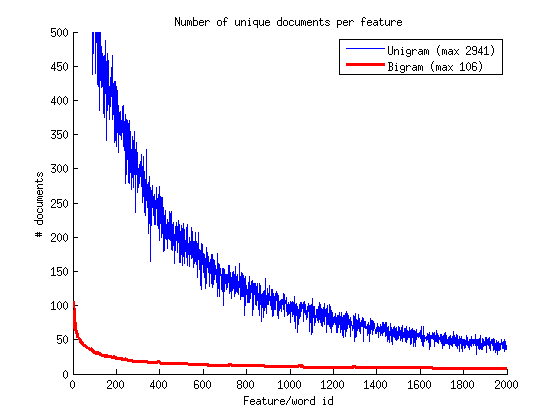
\includegraphics[scale = 0.5]{fig/documents_per_feature.png}
\caption{Documents per feature}
\label{fig:docperfeature}
\end{figure} \\

%Feature values corresponds to the term occurrence frequencies.
%The calculation for this was done in a number of steps.

%The text categorization was implemented in python. Feature values was generated
%for both 1-grams and 2-grams to be able to see if a n-gram, $n > 1$, improves
%the result when running the classification algorithms.

%The output data is represented by a matrix $(words \times document)$ where each
%elements represents the TF-IDF value for the frequency of a word in a specific
%document.
%It's obvious for one to realize that it isn't possible to take all unique words
%into account since the output matrix would have been enormous if so was the
%case. Even further it's not obvious that the classification results gets better
%just because every word is taken into account. Therefor several tests was
%performed using different number of features or more specific words or bigrams
%in this case.

%Stop-words \\
%TF-IDF \\
%Snowball, $https://pypi.python.org/pypi/PyStemmer/1.1.0$ \\
%Ta bort tecken
%ngrams
\section{Naive Bayes}

Naive Bayes was implemented using the prior probabilities $P(x_i\vert c)$ used in the Naive Bayes model $P(c\vert\mathbf{x})$, defined previously in Equation \ref{eq:naivebayes_model}. These were interpreted as the individual probabilities of each word $w$ from a vocabulary $\mathbf{V}$ occurring in class $c$, by exchanging $\left\{x_i : 1 \le i \le D\right\}$ for $\left\{w_i \in \mathbf{V}\right\}$ when using the model.
\\\\
The implementation of $P(w_i\vert c)$ follows the maximum likelihood estimate of relative frequency as follows:
\begin{align}
P(w_i\vert c) =
\frac
	{
		\sum_{d \in \mathbf{D}} F_{w_i}^{(d)}
	}
	{
		\sum_{w_j' \in \mathbf{V}} \sum_{d \in \mathbf{D}}  F_{w_j'}^{(d)}
	},
\end{align}
where $F_w^{(d)}$ defines the relative word frequency in document $d$ from corpus $\mathbf{D}$, implemented with the following two options to be compared:
\begin{description}
  \item[Binary frequency:] Boolean $\in \left\{0,1\right\}$ if word $w$ occurs in document $d$,
  \item[Tf-idf:] $\frac{\texttt{Normalized term frequency}}{\texttt{Document frequency}} \in \left[0, \log \left\vert \mathbf{D}\right\vert\right]$.
\end{description}
A caveat with this procedure is that since both of these options allow for $F_{w_i}^{(d)}$ to be zero, the product in the Naive Bayes model (\ref{eq:naivebayes_model}) for $P(c\vert d)$ vanishes for all combinations of classes $c$ and documents $d$ for which $d$ includes a word $w_i$ that never occurs in the given class. To assure nonzero prior probabilities Laplace smoothing was used, which adds one to each count as follows \citep{nb_ref}. 

\begin{align}
P(w_i\vert c) =
\frac
	{
		1 + \sum_{d \in \mathbf{D}} F_{w_i}^{(d)}
	}
	{
		\left\vert\mathbf{V}\right\vert + \sum_{w_j' \in \mathbf{V}} \sum_{d \in \mathbf{D}} F_{w_j'}^{(d)}
	},
\end{align}
The parameter $P(c)$ is implemented as
\begin{align}
P(c) = \frac{\left\vert\mathbf{D}_c\right\vert}{\left\vert\mathbf{D}\right\vert}
\end{align}
where $\left\vert\mathbf{D}_c\right\vert$ is the number of documents with class $c$. The training algorithm is shown in Algorithm \ref{algorithm:naive_bayes_training}.\\\\\\\\\\\\\\\\\\\\\\\\\\\\\\\\\\\\\\

\begin{algorithm}[h]
 \SetAlgoLined
 
 \KwData{\textit{Word Tf-idf-values} $\left\{F_{w_i}^{(d)} : d \in \mathbf{D}, 1 \le i \le \left\vert\mathbf{V}\right\vert\right\}$;
 		 \textit{Training classes} $\left\{c_d : d \in \mathbf{D}, c \in \mathbf{C}\right\}$; \textit{Using Tf-idf boolean} \texttt{use\_tfidf}}
 \KwResult{$P(c), P(w\vert c)$}
  \For{$i=1$ \KwTo $\left\vert\mathbf{C}\right\vert$}
  {
  	class $\leftarrow c_i$\\
  	P(class) = $\frac{\left\vert\mathbf{D}_c\right\vert}{\left\vert\mathbf{D}\right\vert}$
  }
 \ForEach{$d \in \mathbf{D}$}
 {
	class $\leftarrow c_d$\\
	\For{$i=1$ \KwTo $\left\vert\mathbf{V}\right\vert$}
	{
		word $\leftarrow w_i$ \\
		\uIf{\texttt{use\_tfidf}}
		{
			$P($word$\vert$class$)$ += $T_{w_i}^{(d)}$
		}
		\Else
		{
			$P($word$\vert$class$)$ += $1$
		}
	}
 }
 Normalize($\left\{P(w\vert c) : w \in \mathbf{V}, c \in \mathbf{C}\right\}$)\\
 \Return $\left\{P(c), c \in \mathbf{C}\right\}, \left\{P(w\vert c) : w \in \mathbf{V}, c \in \mathbf{C}\right\}$
 \caption{Multinomial Naive Bayes training algorithm}
 \label{algorithm:naive_bayes_training}
\end{algorithm}


\section{K-Nearest Neighbour (KNN) algorithm}
The KNN algorithm was implemented by interpreting each feature, or in this case
every document, as a dimension and feature values corresponds to the term
occurrence frequencies. Calculations of the nearest neighbours were
implemented in a non deterministic way. This because of that a point $x$ in a plane
may have neighbours with the property that they have equal distances to
$x$. If this is the case a nearest neighbour is chosen at random. Several choices
for $k$ were tested in different runs of the algorithm to find the best $k$ for
the classification. The algorithm was implemented to be able to classify both
different classes (music , software, etc.) and sentimental classification
(positive, negative). Figure \ref{fig:KNNplot} shows the misclassification done by the
algorithm for both different $k$ and different sizes of the feature sets. The plot was generate with training set size 2000 and test set size 100 for unigrams. Note that the result might look different for other training set sizes. We used the best $k$ from this plot which is full training set size.
\begin{figure}[h!]
\centering
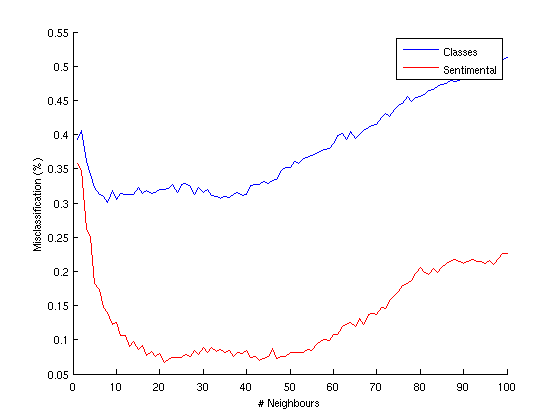
\includegraphics[scale=0.6]{../Plottar/knn_2000words_testdata100_unigram}
\caption{Plot showing results from the KNN classifier}
\label{fig:KNNplot}
\end{figure}\\
Figure \ref{fig:KNNplot} shows that KNN has best performance with parameter $K = 20$ for sentimental and $K = 10$ for classes.

%\begin{comment}
%The pseudocode below described the implemented matlab code.

%\begin{algorithm}[H]
% \SetKwData{Left}{left}\SetKwData{This}{this}\SetKwData{Up}{up}
% \SetKwFunction{Union}{Union}\SetKwFunction{FindCompress}{FindCompress}
% \SetKwInOut{Input}{input}\SetKwInOut{Output}{output}
% \Input{A data set X, A vector of labels Y,Number of nearest neigbour k,A feature vector x}
% \Output{A classification index}
% $\forall$ documents in data calculate the distances $D$ to $x$\;
% SDI = Sort the vector D and get the indexes in D \;
% S = A zero vector of size equal to the number of labels \;
%
% \For{i $\in$ \{1 \ldots k\}}{
%  read current\;
%  \eIf{understand}{
%   go to next section\;
%   current section becomes this one\;
%   }{
%   go back to the beginning of current section\;
%  }
% }
% \caption{How to write algorithms}
%\end{algorithm}


\section{Support Vector Machine (SVM)}
The pre-implemented Support Vector Machine used the matlab library $svmtrain$ \citep{svmtrain_ref}, from the Statistics toolbox, seen in Algorithm~\ref{algorithm:SVM}.  Svmtrain was configured to be soft margined, penalty parameter $C = 1$, and such that when it did not converge the classification was set to zero, which would represent $100\%$ misclassification. A linear kernel function was used. \\
\begin{algorithm}[H]
\SetAlgoLined
\KwData{Xtraining: The data to train, Ytraining: labels of data to train \\ Xtest: The data to test}
\KwResult{Vector containing the classified labels}
\SetKwData{Try}{try}
\SetKwData{Catch}{catch}
\SetKwData{End}{end}
\SetKwIF{Try}{Elseif}{Catch}{try}{:}{else if}{catch:}{}

Set max iterations 150000 \\
\Try{}{
svm$\_$model = $svmtrain(Xtraining, Ytraining, linear)$ \\
classifications = $svmclassify(svm\_model, Xtest)'$
}\Catch{$classifications = zeros( Xtest)$}{}{end}
 \caption{SVM using svmtrain}
 \label{algorithm:SVM}
\end{algorithm}

\section{The Perceptron algorithm}
The Perceptron algorithm was implemented as follows:
The output $w$ from the algorithm was a weight vector with the same size as $y$. If the classification for a $x$ in the training set is equal to $y$, the weight was unchanged.
If $y$ was 1 and the classification -1, then $w$ was increased. If $y$ was -1 and the classification 1, then $w$ was decreased \citep{perceptron_ai}. Algorithm~\ref{algorithm:perceptron} shows the pseudocode for the Averaged Perceptron. The Averaged Perceptron and the usual Perceptron works in the same way except that the Averaged Perceptron returns the average weight vector $wa$ instead of the final $w$.
This averaged vector was built incrementally by updating it while the usual weight vector was built. The pseudocode is almost the same as for the usual perceptron.
\begin{algorithm}[h!]
 \SetAlgoLined
 \KwData{Xtraining: The data to train, Ytraining: labels of data to train}
 \KwResult{Weight vector $wa$}
 Initialize weight vector $w$ and averaged weight vector $wa$ to all zeros\;
 Initialize the counter $c$ to 0\;
 $N \leftarrow$ number of iterations through training set\;
 \For{1 $\rightarrow$ N}{
   \ForAll{x in Xtraining, y in Ytraining}{
    $guess \leftarrow sign(x \cdot w)$\;
    \If{$guess \neq y$}{
     $w \leftarrow w + (y \cdot x)$\;
     $average\_weight \leftarrow (N\cdot T - c) / (N\cdot T)$\;
     $wa \leftarrow wa + average\_weight \cdot (y \cdot x)$\;
     }
     Increase the counter $c$\;
     
   }
 }
 \Return $wa$
 \caption{Averaged Perceptron}
 \label{algorithm:perceptron}
\end{algorithm} \\
In both the Perceptron algorithms, the algorithm makes a number of iterations. To decide how many iterations that must be done to get a fair result the misclassifications and the number of iterations were plotted, which is shown in Figure~\ref{fig:number_iterations}. The algorithms used input data of 2000 words (unigram) and 10-fold crossvalidaion. As seen in the plot, both the algorithms converged after around 15 iterations for both sentimental classification and the classification for different classes. 
\begin{figure}[h!]
\centering
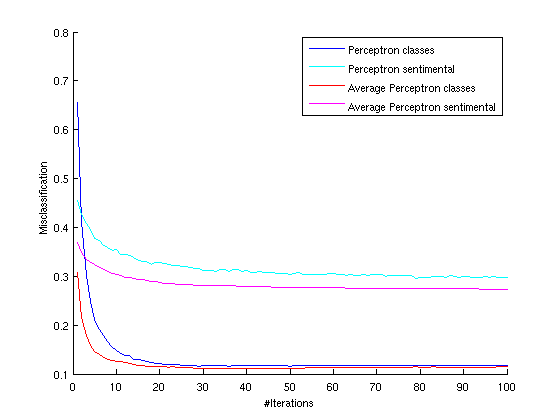
\includegraphics[scale = 0.5]{../Plottar/perceptron_2000words_unigram_10foldcv_classes-high_sentimental-low.png}
\caption{Plot over misclassifications for different \#iterations}
\label{fig:number_iterations}
\end{figure}\\
Since the Perceptron algorithms are 0/1 classifiers there were some difficulties with classifying the data as classes. This was solved by: for all data and all classes classify if data belongs to this class or not. Finally choose the class it belonged to most.
